\section{l'évolution d'Hadoop}
Depuis sa création, Hadoop a constamment évolué avec des mis à jour régulière. Sa dernière version à ce jour étant l’Ozone release 0.2.1-alpha. Mis à part la correction des bugs, chaque nouvelle version apporte de nouveaux modules et fonctionnalités. Ozone est un magasin de d’objet sémantiques clé-valeur pouvant gérer à la fois des fichiers volumineux et moins volumineux. Depuis sa sortie initiale, les versions 0.20.x étaient les premières à être considéré comme stable, pouvant être utilisé dans un environnement de production. Les versions 0.23.X on inclus deux caractéristiques majeures à savoir la version actuelle de Hadoop NextGen MapReduce également connu sous le nom de YARN. En 2011 Hadoop sort la version 1.0.0 qui incluait le webHDFS et des fonctionnalités de sécurité sur HBase. En mai 2012, Hadoop 2.0.x est publié et le 2.0.0-alpha inclus des fonctionnalités majeures importantes sur la sérié 1.x. dérivé de la branche 0.23.x. Les caractéristiques les plus importantes inclues étaient HDFS HA (High Availability), fédération ARN et HDFS. Cette version est considéré comme une version consolidé de la branche0.23.x. Les branches 1.x et 2.x sont les branches principales des versions Hadoop et ont des déférences significatives. Pour le premier, il s’agit de l’introduction du YARN(Nextgen MapReduce initialement présent sur les version 0.23.x). YARN propose la séparation entre deux fonctions majeur du JobTra-cker : gestion des ressource et planification/ surveillances des travaux.

Dans la version 2.x, YARN et plateforme de gestion d’application distribuée tandis que Hadopp MapReduce reste une plateforme de traitement distribué. L’autre inclusion est le HDFS HA, qui favorise la haute disponibilité de HDFS. Avant la version 2.0.0 Namenode était un point unique d’échec dans un cluster HDFS. Un échec sur la machine Namenode rendrait l’ensemble du cluster HDFS indisponible. La troisième fonctionnalité est le HDFS Fendra qui prend en charge plusieurs Namenodes dans un système de fichier HDFS. Théoriquement, bien que supporté dans les versions 2.x, la différence avec la version 1.x se creuse et ne sera peut-être plus prise en charge. \cite{polato_comprehensive_2014}
\begin{figure}
  \begin{center}
  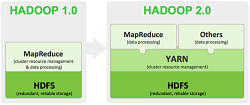
\includegraphics{images/hadoop-evolution.png}
    \end{center}
    \caption{évolution d'Hadoop par https://www.lebigdata.fr/hadoop}
    \label{fig:https://www.lebigdata.fr/hadoop}
\end{figure}